\documentclass{llncs}
\usepackage{listings}
\usepackage{color}
\usepackage{graphicx}

\lstset{basicstyle=\scriptsize\sffamily}
%\lstset{language=Assembler}[avr8avra] % not standard
\lstdefinestyle{customasm}{
  morekeywords={adc,adiw,asr,brts,brcs,brhs,brne,cbr,clh,clr,clt,cp,cpi,dec,eor,ldi,lpm,lsl,nop,mov,or,rcall,ret,seh,set,subi,swap,rjmp},
  morecomment=[l][\color{blue}]{;}
}
\lstset{style=customasm}

\begin{document}

\title{Speed and size-optimized implementations of the PRESENT cipher for AVR machines}
\author{
Kostas Papagiannopoulos \\
Aram Verstegen
}
\institute{Radboud Universiteit Nijmegen}
\date{\today}

\maketitle

\abstract{
We present our progress in experimenting with the PRESENT block cipher to optimize it for the AVR architecture in both the direction of speed and area.}

\section{PRESENT}
PRESENT \cite{bogdanov2007present} is an ultra-lightweight 64-bit block cipher using 80-bit or 128-bit keys based on a substitution/permutation network.
\begin{figure}
	\label{present_schematic}
	\caption{Schematic of the PRESENT cipher}
	\centering 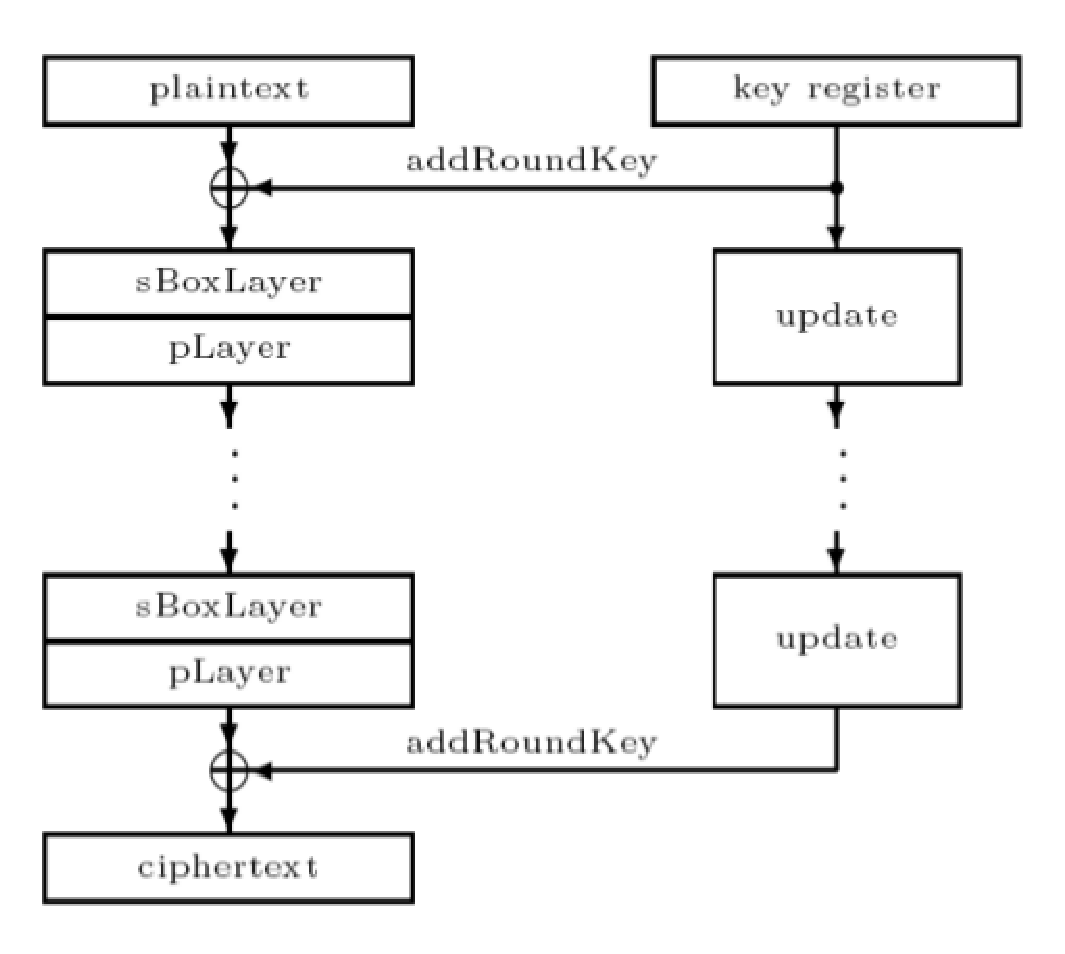
\includegraphics[width=0.4\textwidth]{present.eps}
\end{figure}


PRESENT was adopted by ISO as a standard for a lightweight block cipher. \cite{present_iso}

PRESENT uses exclusive-or as a round key, a 4-bit substitution layer and a 4-bit period bit position permutation network in 31 rounds, and a final round key.
Key scheduling is a combination of bit rotation, S-box application and exclusive-OR with the round counter.
We chose PRESENT as a cipher to work on within a project to write and optimize AVR crypto code because we deemed it extremely well-suited for a simple microcontroller, and felt it was within our grasp to implement and optimize correctly within the allotted time.

Constructs found in PRESENT are also used in the SPONGENT \cite{bogdanov2011spongent} hash function, so the optimizations we present here might also interest SPONGENT implementers.

We have implemented PRESENT for 80-bit keys in AVR assembly and optimized for speed and size.

%The coursework asked us to draft optimized implementations in the direction of speed and code size, and these constraints also drove us to .
%by providing one faster implementation, and one smaller implementation to complement their version which strikes a balance between the two.
%We were already underway implementing the algorithm in a high-level language to understand it better when we learned of the work done by Leuven University's project group to implement PRESENT and other light-weight ciphers for AVR machines \cite{eisenbarth2012compact}.
%Although we felt it would be bad sportsmanship to peek at the code before we had some AVR code up and running, by the time we needed to implement the permutation layer our curiosity was hard to temper.
%Meanwhile we had also found 

%\section{Algorithm}

The first 64 bits of the 80-bit key register form the round key.
This key register is supplied with the 80-bit cipher key.
To encrypt one 64-bit block, each encryption round PRESENT applies an XOR with the current round key followed by substitution and permutation layer.
The substitution layer applies nibble-wise (4-bit) S-boxes to the state, the permutation layer re-arranges the bits in the state following a 4-bit period.
Key scheduling is done by rotating the key register 61 bit positions to the left, applying the S-box to the top nibble of the key register and XORing bits 15 through 19 with the round counter.
There are a total of 31 of these rounds in 80-bit PRESENT, and finally the round key is applied one last time.
(See Figure~\ref{present_schematic})


\section{Speed optimizations}
\subsection{PRESENT S-Box}\label{sbox}
In this section we examine the S-Box of the PRESENT cipher from the speed perspective and we view it as a standalone component. We start from the original S-Box, identify its performance issues (section \ref{osbox}) and we expand it to the more efficient Squared S-Box (section \ref{ssbox}). Based on these improvements, we examine the S-Box and permutation layer combined  in section \ref{msbox}.
\subsubsection{Original S-Box}\label{osbox}
The original S-Box, presented by Bogdanov et al.~\cite{bogdanov2007present} consists of 16 different S-Boxes, each with a 4-bit input and a 4-bit output, as show below.\\
\begin{table}[h]
\centering
\begin{tabular}{| c | c  | c | c | c  | c | c | c  | c | c | c  | c | c | c  | c | c | c |}
\hline
  x & 0 & 1 & 2 & 3 & 4 & 5 & 6 & 7 & 8 & 9 & A & B & C & D & E & F   \\
\hline
  S-Box[x] & C & 5 & 6 & B & 9 & 0 & A & D & 3 & E & F & 8 & 4 & 7 & 1 & 2   \\
\hline
\end{tabular}
 \caption{\small The original S-Box of the PRESENT cipher.}
\end{table}


The core issue with the 4-bit S-Box is the penalty in accessing it, if stored in a lookup table. The AVR architecture is designed to enable fast access for 8-bits at a time. Thus, a lookup table with of the original S-Box is rather small (16 bytes for an unpacked version, 8 bytes for a packed one), but it is also rather inefficient due to the required shifts and XOR operations that need to take place before and after each table lookup.

\subsubsection{Squared S-Box}\label{ssbox}
A solution to the aforementioned problem is to construct a new lookup table that is custom made for the 8-bit AVR architecture. In the following table, we demonstrate a Squared S-Box, which uses an 8-bit input and produces an 8-bit output. As a result, there is no need for overhead computation and the substitution consists of a single lookup.\\
\begin{table}[h]
\centering
\begin{tabular}{| c | c  | c | c | c  | c  | c | c | c  | c | c | c |}
\hline
  x & 00 & 01 & 02 & 03  &  $\dots$  & 0C & 0D & 0E & 0F   \\
\hline
 S-Box[x] & CC & C5 & C6 & CB & \dots & C4 & C7 & C1 & C2   \\
\hline
  x & 10 & 11 & 12 & 13  &  $\dots$  & 1C & 1D & 1E & 1F   \\
\hline
 S-Box[x] & 5C & 55 & 56 & 5B & \dots & 54 & 57 & 51 & 52   \\

\hline
\end{tabular}
 \caption{\small The first two lines of the 256-byte Squared S-Box. It substitutes one byte at a time, without any overhead.}
\end{table}
The Squared S-Box described, is an efficient and viable solution with respect to the cipher's substitution layer. It is custom made for the 8-bit AVR architecture and allows us to perform byte substitutions with a single FLASH memory lookup. Furthermore, it is relatively size-efficient, consisting of 256 bytes, thus, it can also be transfered to ATtiny45 SRAM from FLASH memory during the initialization process of the algorithm. The memory transfer is viable, since ATtiny45 possesses 256 bytes of SRAM and it will reduce the lookup cost by 33\%, i.e. to perform a lookup, the software will use the \texttt{ld} instruction (load from SRAM - 2 clock cycles), instead of  \texttt{lpm} instruction (load from FLASH memory - 3 clock cycles). The only processing penalty consists of a 256 byte transfer from FLASH to SRAM which will occur only once, preferably in the beginning or setup phase.
\subsection{PRESENT S-Box and Permutation Layer}

Although the Squared S-Box lookup table solution is viable for the PRESENT cipher, we need to stress the fact that the PRESENT cipher possesses a complex permutation layer, requiring a large number of shift and rotate operations. The AVR architecture is not capable of performing fast shifts and rotations,  e.g. an $n$-bit shift requires $n$ clock cycles, and thusly we have to look for alternatives.
\subsubsection{Merged SP Lookup Tables}\label{msbox}
In this direction, work by Peter Schwabe~\cite{hutternacl} on ATmega\footnote{Benchmarking was performed on ATmega2560.} suggested the usage of multiplications instead of rotations/shifts, however this is not viable on ATtiny due to the fact that they do not possess native multiplication instructions. The fastest approach that we identified for the permutation layer is the idea developed by Zheng Gong and Bo Zhu~\cite{gong_code,gong2009towards}. Specifically, they exploited the internal structure of the permutation layer, i.e. the fact that every output of a 4-bit S-Box will contribute one bit to the cipher (the underlying pattern for the permutation is the following: $for$ $k:old$ $position,$ $l:new$ $position,$ $l=f(k)=16(k mod 4)+(k div 4)$ ). Thus, the first 2 bits of the output are derived from the first two 4-bit S-Boxes, i.e. from the first byte of the previous state. \\
Using these observations, they crafted four 256-byte lookup tables (1024 bytes in total) that \emph{merge} the S-Box and the permutation layer and as a result, the whole SP network is performed via table lookups. On the downside, we have to perform one lookup for every two bits, resulting in 32 lookups for a 64-bit state (compared to the Squared S-Box that required only 8 lookups for a 64-bit state). Moreover, we need 1024 bytes to store the tables, thus it is not possible to transfer them to the SRAM. The 33\% speedup obtained in section \ref{ssbox} is only possible in an AVR microcontroller with at least 1024 bytes of internal\footnote{Additional external SRAM is not an option, since it is at least as slow as FLASH memory.} SRAM, for instance ATtiny1634.

\subsubsection{Fast Lookup Table Access}
In order to decrease the computational penalty of the table lookups, we performed several code-level optimizations. Below, we demonstrate the code required to perform a single table lookup from FLASH memory.

\begin{figure}
\begin{lstlisting}
LookupTable_i:
mov ZH, high_part_of_address_i ; load ZH with the 8 high bits
mov ZL, low_part_of_address_i  ; load ZL with the table index
lpm Rd, Z                      ; load register d with Table[ZL] contents
\end{lstlisting}
	\caption{Fast S-box table access.}
\label{sbox_squared}
\end{figure}
We aim to keep the changes required in \texttt{ZH} to a minimum. Thus, we align the four 256-byte tables such that they can be accessed by using only the  \texttt{ZL} register as an index and keeping \texttt{ZH} unchanged. Elaborating, the four lookup tables \texttt{LookupTable3, LookupTable2, LookupTable1, LookupTable0} (section \ref{msbox}) start from \texttt{0x0600, 0x0700, 0x0800, 0x0900} respectively and thus, the 8 high bits of the address part (\texttt{0x06, 0x07, 0x08, 0x09}) remain the same and the 8 low bits can act as the table index, ranging from 0 to 255 (\texttt{0x00} to \texttt{0xFF}). \\
To similar end, we group lookups that search in the same table, as follows.
\begin{figure}
\begin{lstlisting}
LookupTable_0 ;	                LookupTable_0 ; Group 0 
LookupTable_1 ;	                LookupTable_0 ; Group 0
LookupTable_0 ;  transforms to  LookupTable_1 ; Group 1
LookupTable_1 ;	                LookupTable_1 ; Group 1
\end{lstlisting}
	\caption{Batched lookup table access.}
\label{batched_lookup}
\end{figure}
We perform the maximum amount of grouped table lookups, given the limited number of registers. Withing each grouping, \texttt{ZH} remains the same.
\subsection{Key Update Function}
They key update function of the PRESENT cipher consists of three operations, namely, key rotation, key substitution and key XOR the round counter. We present the optimizations performed below.
\subsubsection{Key Rotation Operation}
The algorithm specifies that the key must be rotated by 61 bits to the left. Given the fact that rotations/shifts are computationally expensive, we transform 61 left rotations to 19 right rotations, which can be further reduced to 16 right rotations and 3 right rotations. The 16 right rotations can be easily performed with the \texttt{mov} instructions and the 3 remaining are carried out with the \texttt{ror} and \texttt{shr} commands.
\subsubsection{Key Substitution Operation}
The highest 4 bits of the 80-bit key used by PRESENT cipher, must go through the S-Box. To avoid again 4-bit memory access, we craft another Squared S-Box that substitutes the 4 high bits of the 8-bit input, while the low 4 bits remain unchanged. The resulting table can be seen below and the key substitution operation consists of a single lookup.

\begin{table}[h]
\centering
\begin{tabular}{| c | c  | c | c | c  | c  | c | c | c  | c | c | c |}
\hline
  x & 00 & 01 & 02 & 03  &  $\dots$  & 0C & 0D & 0E & 0F   \\
\hline
 S-Box[x] & C0 & C1 & C2 & C3 & \dots & CC & CD & CE & CF   \\
\hline
  x & 10 & 11 & 12 & 13  &  $\dots$  & 1C & 1D & 1E & 1F   \\
\hline
 S-Box[x] & 50 & 5 & 56 & 5B & \dots & 5C & 5D & 5E & 5F   \\

\hline
\end{tabular}
 \caption{Squared S-Box for key substitution, operating only on the high 4 bits of the input.}
\end{table}

\subsubsection{Key XOR Round Counter Operation}
The algorithm specifies that the key bits 15, 16, 17, 18, 19 must be XORed with the round counter. The issue is that -under the current representation- bits 0$\dots$7 will be stored in register0, bits 8$\dots$15 will be stored in register1 and bits 16$\dots$23 will be stored in register2. As a result parts of the round counter need to be XORed with different parts of two separate registers. However, if we perform the XOR operation before the key rotation operation, the bits that will be operated on are bits 34,35,36,37,38 which span a single register (using the previous representation, they are located in register4 ). Performing this operation before the key rotation does not affect the outcome or security of the algorithm.

\subsection{Bitslicing}
NOTE: This is not a valid/verified section yet - we only present thoughts on the possibility of bitslicing. To be reconsidered.\\
Bitslicing has been performed before for PRESENT ~\cite{grabher2008light}.In order to perform bitslicing in AVR, there is need for a large amount of SRAM, e.g. for a fully-blown bitslicing, we need 8*64=512 bytes of SRAM. With this approach we perform 64 encryptions in bitsliced form and we no longer need the permutation layer. On the downside, there will traffic between registers and SRAM and also, we cannot use lookup tables for the substitution layer and thus, we have to implement the S-Box with boolean functions that operate on each state bit.

\section{Size optimizations}

Here we will list some of the size improvements we were able to apply to the PRESENT algorithm.
While these modifications make the algorithm operate more slowly, the reduction in size would allow the cipher to be included in microcontrollers with smaller available code area.
Our version requires 204 AVR instructions (408 bytes of code) for both the encryption and decryption routines, plus two times 8 bytes for packed tables of S-box values at memory addresses \textbf{0x100} and \textbf{0x200}.
We believe this should be sufficiently small for the code to be included in an AVR machine with 1K of available Flash storage, while still allowing over half of the available area to be devoted to application-specific code.

Unfortunately, every opcode in the AVR instruction set is 16-bits wide, so there is nothing to be gained from exchanging any instructions for equivalent smaller ones (such as for example \textit{add Rd, 1} being more concisely expressed as \textit{inc Rd} on x86 machines).
Furthermore the AVR employs a Harvard architecture, where there is a strict separation between data and code memory; this prevents us from dynamically computing new opcodes in memory to be executed later.
Finally we note there are no `bulk' instructions which operate on several registers at once.

However, we do have access to some instructions that are specific to the AVR architecture and are uniquely suited to making parts of the code more condensed by virtue of their expressiveness, such as the \textit{swap} and \textit{cbr} instructions.

\subsection{Serialization}
The biggest size optimization we have implemented is serialization of the algorithm, keeping part of the state in SRAM while we operate on fewer registers.
This reduces the instruction count on all parts of the round update procedure except for key scheduling.

We have chosen to keep 4 bytes of state in registers at a time, as we believe it allows us to apply the permutation layer of the algorithm in software with the most size-efficiency.
Using even fewer state bytes in registers might allow for greater size reductions in other areas of the code, but applying the permutation layer may turn out to be more troublesome in that case.
%We would of course welcome efforts from the community to disprove this assumption.

\subsection{S-box packing}
The PRESENT S-boxes work on 4-bit nibbles, but defining a table of nibbles in the code at first seemed less size-efficient than packing the nibbles into bytes to be unpacked.
This would save 8 bytes per S-box table to start with, but we need 5 to 8 instructions in stead of a \textbf{ld} (load) depending on whether or not we care about timing attacks to unpack the nibbles which diminishes the size benefit to 2 bytes of code. See Figures~\ref{unpacking_code} and \ref{packed_sbox}.
%We consider this a fair loss for our optimization strategy, and also see an upside: having the S-boxes unpacked as data improves throughput and makes the encryption and decryption code smaller to distribute separately.
%We decided 2 bytes of area reduction just wasn't worth the other losses.
%The packed table approach is therefore only beneficial when we require encryption and decryption routines in the target application, in which case it would save the remaining 6 bytes.

\begin{figure}
	Before: \\
	\begin{tabular}{ | c | c | c | c | c | c | c | c | c | c | c | c | c | c | c | c | }
	  \hline                        
	  C & 5 & 6 & B & 9 & 0 & A & D & 3 & E & F & 8 & 4 & 7 & 1 & 2 \\
	  \hline  
	\end{tabular}
	\\

	After: \\
	\begin{tabular}{ | c | c | c | c | c | c | c | c | }
	  \hline                        
	  C5 & 6B & 90 & AD & 3E & F8 & 47 & 12 \\
	  \hline  
	\end{tabular}
	\caption{Packing of S-box nibbles initially saves 8 bytes.}
	\label{packed_sbox}
\end{figure}

\begin{figure}
\begin{lstlisting}
	unpack_sBox:
		asr ZL                ; halve input, take carry
		lpm SBOX_OUTPUT, Z    ; get S-box output
		brcs odd_unpack       ; branch depending on carry
	even_unpack:
		swap SBOX_OUTPUT      ; swap nibbles in S-box output
		rjmp unpack
        odd_unpack:
                nop                   ; guard against timing attacks
                nop
        unpack:
                cbr SBOX_OUTPUT, 0xf0 ; clear high nibble in S-box output
	\end{lstlisting}
	\caption{Unpacking bytes into nibbles in a constant cycle count takes us 8 instructions whereas unpacking unpacked nibbles takes us only 1. The net gain is only 2 bytes of code.}
\label{unpacking_code}
\end{figure}



\subsection{Permutation layer}
The code to apply permutations to the state in software borrows heavily from the AVR implementation of PRESENT drafted in Leuven by Eisenbarth et al \cite{eisenbarth2012compact}.
Since the permutation follows a 4-bit period in the input it seems most efficient to use 4 bytes of I/O when rotating bits off of registers into corresponding new positions.

In the Leuven implementation one bit is rolled off from 4 state registers into one output register and this block is done twice, completing one output byte. It has made ingenious use of the side-effect that both the input and the output are being rotated, allowing the operation to be reversed depending on the offset at which the procedure is called.

\subsection{Branching on SREG flags}
A subtle but real size optimization we implemented focused on the code used to drive repeated operations .
The construct in Figure~\ref{sreg_redo} allows the implementer to let a block of code be executed twice, while allowing them to take control of the machine before, after and in between these code blocks.
In our implementation this has been applied to the substitution and permutation layer procedures to save a few instructions.
This does not affect the cycle count relative to the state or input.
This construct also allows the \textit{unpack\_sBox} code we just defined to be inlined into our S-box procedure, saving 2 more instructions.

\begin{figure}
	\begin{lstlisting}
	setup_redo_block:
		clt                   ; clear T flag
		rjmp redo_block       ; do the second part
	block:
		set                   ; set T flag
		; fall through
	redo_block:
		; instructions here happen twice when called from block

		brts setup_redo_block ; redo this block? (if T flag set)
		ret
	\end{lstlisting}
	\caption{A construct that uses the state register to re-do a block twice with code executing before, after and in between, allowing more code to be inlined.}
\label{sreg_redo}
\end{figure}

We have used this construct in the procedures for both steps of applying the SP-network while retaining the property that these procedures can be called from two different offsets.

The S-box substitution procedure for example replaces only the high nibble when called from one offset, and the whole byte when called from another.
The code to swap a byte simply re-uses a nibble-wise operation while swapping the nibbles before and after to complete an entire byte.

In the permutation procedure the operations on 4 input bits is done twice, to complete one output byte.

\subsection{Keying and key scheduling}
Because we have serialized part of the algorithm our key register needs to be rotated when changing the context between steps that apply to the higher and lower 4 bytes of the cipher's state.
Because we required a procedure to rotate the key register for key scheduling anyway, that code can be reused for this purpose, and we can still apply the exclusive-or to part of the key register in the ideal position (i.e. where the bytes of the key register line up with the round counter register).

The inverse key scheduling procedure is only needed in the decryption routine, so we were able to inline it into the decryption round and combine the operations for key scheduling and rotating the register to the appropriate position for the next round.

\subsection{Reducing code size for specific applications}
While the attained size of the implementation of PRESENT should suffice for use in real-world applications, some of the input and output procedures as well as the S-box unpacking code can be omitted when only encryption or encryption is required in the application.
This is highlighted in the source code using comments.

\section{Conclusion}
We've compared our results to the existing AVR implementation by Eisenbarth et al \cite{eisenbarth2012compact} and are pleased to announce we were able to halve the code size and gain about 13\% speed increase.
We note that having access to a larger SRAM could allow the lookup tables for the speed-optimized version to incur a lower overhead, and reduce an estimated 10\% more cycles per encryption. 
\\

	\begin{tabular}{ l | c | c | c }
                & Reference & Speed optimized & Size optimized \\
        Size (bytes) & 936 & 1794 & 426 \\
        Encryption (cycles) & 10723 & 8721 & 90725 \\
        Decryption (cycles) & 11239 & - & 102257 \\
        RAM (bytes) & 0 & 18 & 18
	\end{tabular}

%\section{References}
\bibliography{PRESENT_size_optimized_paper}{}
\bibliographystyle{plain}

\end{document}

